\documentclass[twocolumn,10pt,a4paper]{article}

\usepackage[utf8]{inputenc}
\usepackage[T1]{fontenc}
\usepackage[french]{babel}
\usepackage{mathptmx}
\usepackage{amsmath,amssymb}
\usepackage{graphicx}
\usepackage{booktabs}
\usepackage{listings}
\usepackage{xcolor}
\usepackage[margin=2cm,columnsep=0.7cm]{geometry}
\usepackage{caption}
\usepackage{hyperref}
\hypersetup{hidelinks}

\captionsetup{font=small,labelfont=bf}
\setlength{\parskip}{0pt}

\usepackage{stfloats}
% flottants : laisser plus de place sur les pages de texte et densifier les
% pages de figures, pour qu'elles ne s'accumulent pas en fin de document et ne
% viennent pas couper la bibliographie
\renewcommand{\topfraction}{0.92}
\renewcommand{\bottomfraction}{0.85}
\renewcommand{\textfraction}{0.06}
\renewcommand{\floatpagefraction}{0.7}
\renewcommand{\dbltopfraction}{0.92}
\renewcommand{\dblfloatpagefraction}{0.7}
\setcounter{topnumber}{3}
\setcounter{dbltopnumber}{3}
\setcounter{totalnumber}{5}

\lstset{
  basicstyle=\ttfamily\footnotesize,
  keywordstyle=\color{blue!60!black},
  commentstyle=\color{green!45!black},
  numbers=none, frame=single, framesep=3pt, rulecolor=\color{gray!40},
  breaklines=true, showstringspaces=false, language=Python, aboveskip=4pt, belowskip=2pt,
}

% pourcentages (sans le signe), mis a jour depuis results/*.json apres entrainement
\newcommand{\stlbase}{42{,}2}
\newcommand{\stlbest}{53{,}3}
\newcommand{\neuref}{78{,}9}
\newcommand{\neufull}{90{,}6}
\newcommand{\neulossA}{3{,}03}
\newcommand{\neulossB}{0{,}85}
\newcommand{\neueffmae}{73{,}1}
\newcommand{\neueffrnd}{53{,}3}

\title{\vspace{-2.2em}\textbf{\large Masked Autoencoder implémenté à la main :\\
pré-entraînement auto-supervisé et classification de défauts de surface}}
\author{Philémon Vittet\\ \small Cours d'introduction à la computer vision\\
\small Code : \url{https://github.com/PhilV1tt/mae-from-scratch}}
\date{}

\begin{document}
\maketitle

\begin{abstract}
\noindent
\small
Ce rapport décrit la réimplémentation complète d'un Masked Autoencoder (MAE) sans
différentiation automatique ni couches préfabriquées. Le passage avant et la rétropropagation
de chaque couche, attention et normalisation comprises, sont dérivés et codés à la main, puis
validés par différences finies (erreur relative inférieure à $10^{-6}$). torch n'est utilisé que
comme bibliothèque de tableaux, ce qui permet d'exécuter ces opérations manuelles sur GPU (Apple
MPS) et donc d'entraîner dans des temps raisonnables. Le modèle est étudié sur STL-10, où l'ablation du
taux de masquage illustre l'étude centrale de l'article d'origine, puis appliqué à la
classification de six défauts de surface d'acier (jeu de données NEU). Pré-entraîné sans
étiquettes, son encodeur gelé alimente une sonde linéaire qui atteint $\neufull\,\%$ d'exactitude,
contre $\neuref\,\%$ pour un encodeur non entraîné ; l'écart se creuse quand peu d'images sont
étiquetées.
\end{abstract}

\begin{figure*}[t]
\centering
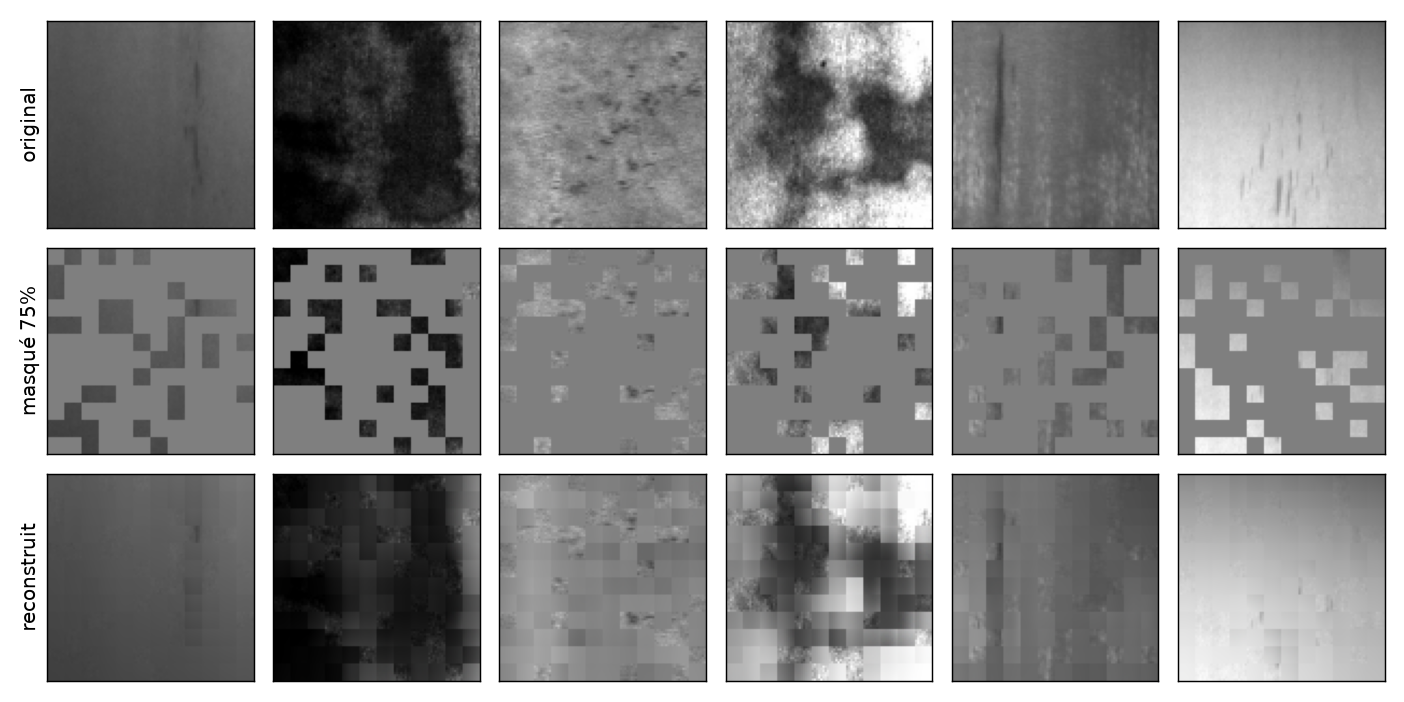
\includegraphics[width=0.86\textwidth]{figures/neu_reconstruction.png}
\caption{Le MAE appliqué aux défauts de surface d'acier. À partir des 25\,\% de patchs visibles
(ligne du milieu), le décodeur reconstruit l'image (ligne du bas) ; l'encodeur ainsi pré-entraîné,
sans étiquettes, sert ensuite à classer le type de défaut.}
\label{fig:teaser}
\end{figure*}

\section{Introduction}

Le coût de l'annotation est un frein récurrent en vision industrielle : étiqueter des défauts
demande un opérateur expert, et chaque ligne de production change la distribution des images.
L'apprentissage auto-supervisé permet de réduire ce coût, en apprenant des représentations sur des
images non étiquetées avant de n'utiliser les étiquettes que pour une tâche aval légère.

Le Masked Autoencoder \cite{he2022mae} masque une grande partie des patchs d'une image et entraîne
un Transformer à reconstruire les pixels manquants. Ce travail vise trois objectifs. Comprendre le
MAE en le réimplémentant intégralement, ce qui impose de dériver à la main la rétropropagation de
l'attention et de la normalisation, plutôt que de s'appuyer sur l'autograd d'un framework. Vérifier
ensuite, sur STL-10, que le pré-entraînement apprend des représentations utiles, mesurées par sonde
linéaire, et observer l'effet du taux de masquage. Appliquer enfin la méthode à un jeu de données
industriel de défauts d'acier et évaluer son intérêt quand les étiquettes sont rares.

\section{Travaux liés}

Le MAE prolonge les autoencodeurs débruiteurs \cite{vincent2010dae} et transpose à l'image la
modélisation masquée de BERT \cite{devlin2019bert}, où seules les positions masquées contribuent à
la perte. Son ossature est le Vision Transformer \cite{dosovitskiy2021vit}, qui découpe l'image en
patchs et applique un Transformer \cite{vaswani2017attention}. BEiT \cite{bao2021beit} prédisait des
tokens discrets ; le MAE montre qu'il suffit de reconstruire les pixels. La détection de défauts de
surface repose aujourd'hui sur des réseaux convolutifs et des détecteurs profonds
\cite{bhatt2021,tang2023} ; le jeu de données NEU \cite{song2013,he2020} en est une référence. Ces
méthodes sont supervisées, là où le pré-entraînement auto-supervisé étudié ici cherche à réduire le
besoin d'étiquettes.

\section{Méthode}

\paragraph{Tokenisation.}
Une image $96\times 96$ est découpée en patchs $8\times 8$, soit une grille $12\times 12 = 144$
patchs aplatis en vecteurs de dimension $8\cdot 8\cdot 3 = 192$, projetés linéairement vers une
dimension d'embedding $D$. On ajoute un encodage positionnel sinusoïdal 2D fixe : l'auto-attention
est invariante à l'ordre, sans position le modèle ne sait pas où se situe chaque patch. Le choix de
patchs $8\times 8$ plutôt que $16\times 16$ divise par deux la taille du bloc reconstruit et réduit
nettement l'aspect en damier des reconstructions, au prix d'une séquence quatre fois plus longue.

\paragraph{Masquage.}
Pour chaque image, un bruit aléatoire sur les 144 positions est trié, ce qui fournit une
permutation. Les $N_{vis} = \lfloor 144\,(1-r)\rfloor$ premiers patchs sont conservés et les autres
masqués, $r$ étant le taux de masquage. Les indices de restauration sont mémorisés pour replacer la
séquence dans son ordre d'origine côté décodeur ; la correction du masquage dépend de la cohérence
entre cette permutation et son inverse.

\paragraph{Encodeur et décodeur asymétriques.}
L'encodeur n'applique ses blocs Transformer qu'aux patchs visibles : à 75\,\% de masquage, il ne
traite que 36 tokens sur 144, et les tokens masqués n'y entrent jamais. Le décodeur projette les
tokens encodés vers une dimension plus étroite, insère un token masqué appris (un vecteur partagé) à
chaque position masquée, restaure l'ordre d'origine, ajoute son encodage positionnel, applique
quelques blocs et prédit les pixels de chaque patch par une tête linéaire. Plus petit que
l'encodeur, il n'est utilisé que pour le pré-entraînement.

\paragraph{Perte.}
La cible est l'image découpée en patchs, chaque patch étant normalisé par sa moyenne et son
écart-type. La perte est l'erreur quadratique moyenne sur les seuls patchs masqués :
\begin{equation}
\mathcal{L} = \frac{1}{|\mathcal{M}|}\sum_{i \in \mathcal{M}}
\frac{1}{192}\,\lVert \hat{x}_i - \tilde{x}_i \rVert^2 .
\end{equation}

\paragraph{Sonde linéaire.}
La qualité des représentations est mesurée en gelant l'encodeur, en le passant sur les images
étiquetées sans masquage, en moyennant les tokens (moyennage global) en un vecteur par image, puis
en entraînant un unique classifieur linéaire par régression logistique \cite{he2022mae}. La
référence est le même protocole sur un encodeur non entraîné.

\section{Implémentation}

\paragraph{Tout à la main, sur GPU.}
Aucune fonction de différentiation automatique ni de \texttt{torch.nn} n'est utilisée : torch ne
sert que de bibliothèque de tableaux. Chaque couche est une classe qui implémente son passage avant
\emph{et} sa rétropropagation, sur le modèle d'une couche linéaire qui met en cache son entrée. Les
paramètres sont des attributs (\texttt{W}, \texttt{gamma}\dots) et leurs gradients portent le nom
préfixé (\texttt{dW}, \texttt{dgamma}\dots), ce qui permet à l'optimiseur de parcourir le modèle
uniformément. Les couches écrites sont : linéaire, LayerNorm, GELU, attention multi-têtes, MLP, bloc
Transformer pré-norm, encodeur, décodeur et perte. Les deux dérivées non triviales sont celles de la
normalisation (listing~\ref{lst:ln}) et de l'attention, dont le point délicat est la jacobienne du
softmax, les logits ayant été mis à l'échelle par $1/\sqrt{d_k}$.

\begin{lstlisting}[caption={Rétropropagation manuelle de LayerNorm.},label={lst:ln}]
def backward(self, dy):
    xhat, std = self.cache
    D = xhat.shape[-1]
    self.dgamma = (dy*xhat).reshape(-1,D).sum(0)
    self.dbeta  = dy.reshape(-1,D).sum(0)
    dxhat = dy * self.gamma
    dx = (dxhat - dxhat.mean(-1,keepdim=True)
          - xhat*(dxhat*xhat).mean(-1,keepdim=True)
          ) / std
    return dx
\end{lstlisting}

\paragraph{Validation des gradients.}
Chaque rétropropagation est vérifiée par différences finies centrées, sur CPU en double précision :
un paramètre est perturbé de $\pm\varepsilon$, la variation de la perte est comparée au gradient
analytique. Sur le MAE complet, la pire erreur relative est inférieure à $10^{-6}$. Ce contrôle est
nécessaire : un gradient erroné ne provoque pas d'erreur d'exécution, il produit seulement un modèle
qui n'apprend pas. Le sur-apprentissage d'un seul batch, masque figé, sert de second test : la perte
y chute, ce qui confirme que le graphe de gradients est correct de bout en bout.

\paragraph{CPU pour vérifier, GPU pour entraîner.}
Le même code tourne sur deux configurations selon l'objectif. Le gradient check exige de la
précision : il s'exécute sur CPU en \texttt{float64}. L'entraînement exige de la vitesse : il
s'exécute sur le GPU Apple (MPS) en \texttt{float32}, où les opérations matricielles écrites à la
main sont environ huit fois plus rapides que sur CPU. C'est ce qui rend abordables les patchs
$8\times 8$ et un modèle de quelques millions de paramètres.

\paragraph{Configuration.}
Le modèle reste modeste (environ $1{,}3$ million de paramètres) ; les hyperparamètres sont donnés
table~\ref{tab:hp}. L'optimiseur est Adam \cite{kingma2015adam} avec weight decay découplé (AdamW
\cite{loshchilov2019adamw}) sur les seules matrices de poids ; le taux d'apprentissage suit une
montée linéaire puis une décroissance en cosinus.

\begin{table}[t]
\centering\small
\begin{tabular}{ll}
\toprule
embedding $D$ & 128 \\
blocs encodeur / décodeur & 6 / 2 \\
têtes & 4 \\
dimension décodeur & 64 \\
ratio MLP & 4 \\
patch / résolution & 8 / $96\times96$ \\
taux de masquage & 0,75 \\
optimiseur & AdamW, $\beta=(0{,}9,\,0{,}95)$ \\
taux d'apprentissage & $8\!\cdot\!10^{-4}$ \\
weight decay & 0,05 \\
taille de lot & 256 \\
époques & 100 (STL) / 600 (NEU) \\
\bottomrule
\end{tabular}
\caption{Hyperparamètres.}
\label{tab:hp}
\end{table}

\section{Protocole expérimental}

STL-10 ($96\times 96$, 10 classes) sert d'étude de méthodologie : pré-entraînement sur 12000 images
non étiquetées, sonde linéaire sur 5000 images étiquetées, évaluation sur 8000 images de test.
NEU-CLS sert de cas applicatif : 1800 images de surface d'acier en six défauts (crazing, inclusion,
patches, pitted surface, rolled-in scale, scratches), en niveaux de gris, dupliquées sur trois
canaux pour réutiliser la même configuration, redimensionnées en $96\times 96$ et réparties de façon
stratifiée en 1440 images d'entraînement et 360 de test. Le MAE est pré-entraîné sans étiquettes,
puis la sonde linéaire est entraînée et évaluée ; le nombre d'images étiquetées fournies à la sonde
est ensuite varié pour mesurer l'apport du pré-entraînement à faible budget d'annotation.

\section{Résultats}

\subsection{NEU : classification de défauts}

Pré-entraîné sans étiquettes sur les images d'acier, le MAE fait décroître la perte de
reconstruction de $\neulossA$ à $\neulossB$ et reconstruit la texture des défauts à partir de
25\,\% des patchs (figure~\ref{fig:teaser}). La sonde linéaire posée sur l'encodeur gelé atteint
$\neufull\,\%$ d'exactitude sur les six défauts, contre $\neuref\,\%$ pour un encodeur aléatoire
(table~\ref{tab:res}). L'apport du pré-entraînement est surtout net à faible budget d'annotation :
l'écart se creuse quand peu d'images sont étiquetées, par exemple $\neueffmae\,\%$ contre
$\neueffrnd\,\%$ avec dix images par classe (figure~\ref{fig:neueff}, gauche). La matrice de
confusion (figure~\ref{fig:neueff}, droite) montre que les erreurs résiduelles concernent surtout
les défauts visuellement proches.

\begin{table}[t]
\centering\small
\begin{tabular}{lcc}
\toprule
& aléatoire & MAE \\
\midrule
STL-10, sonde linéaire (10 classes) & $\stlbase\,\%$ & $\stlbest\,\%$ \\
NEU, sonde linéaire (6 défauts) & $\neuref\,\%$ & $\neufull\,\%$ \\
NEU, 10 étiquettes par classe & $\neueffrnd\,\%$ & $\neueffmae\,\%$ \\
\bottomrule
\end{tabular}
\caption{Exactitude de la sonde linéaire, encodeur aléatoire contre MAE pré-entraîné.}
\label{tab:res}
\end{table}

\begin{figure*}[tbp]
\centering
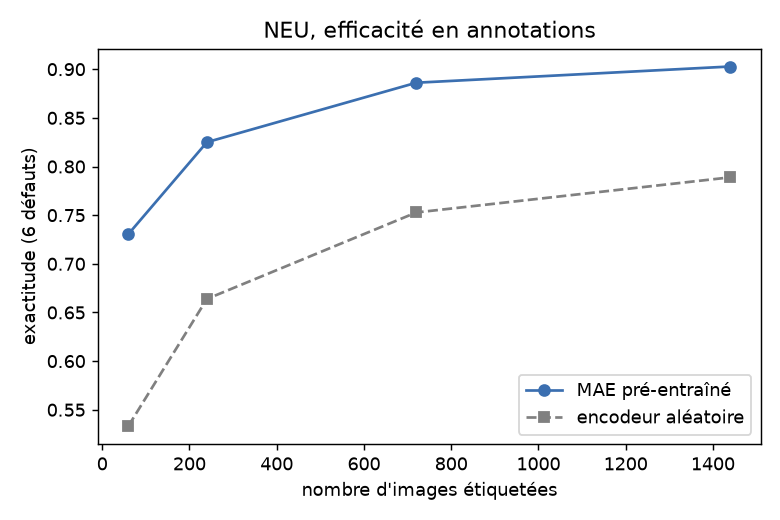
\includegraphics[width=0.45\textwidth]{figures/neu_efficiency.png}
\hfill
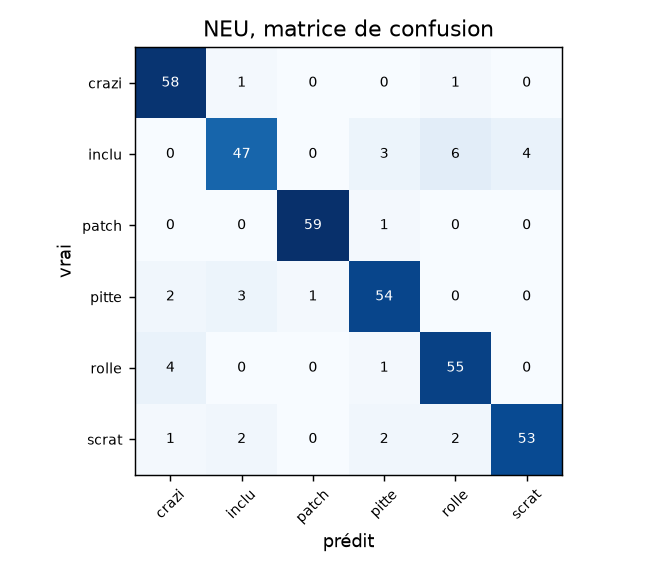
\includegraphics[width=0.38\textwidth]{figures/neu_confusion.png}
\caption{NEU. Gauche : exactitude de la sonde selon le nombre d'images étiquetées, MAE contre
encodeur aléatoire. Droite : matrice de confusion du MAE sur les six défauts.}
\label{fig:neueff}
\end{figure*}

\subsection{STL-10 : ablation du taux de masquage}

Sur STL-10, la reconstruction porte sur des objets variés (figure~\ref{fig:stlrecon}). Le
pré-entraînement fait décroître la perte de reconstruction (figure~\ref{fig:loss}), et la sonde
linéaire dépasse l'encodeur aléatoire, de $\stlbase\,\%$ à $\stlbest\,\%$, ce qui indique que des
représentations utiles ont été apprises. La figure~\ref{fig:probe} reporte l'exactitude selon le
taux de masquage, contre l'encodeur aléatoire et le hasard (10\,\% pour 10 classes).
Les quatre taux dépassent tous l'encodeur aléatoire d'environ dix points, donc le gain
tient surtout au pré-entraînement, pas au réglage fin du masquage. Le maximum est à 0,75
($\stlbest\,\%$), le taux retenu par l'article~\cite{he2022mae}, mais l'écart entre taux reste
faible (51,6 à $\stlbest\,\%$). À cette échelle, la quantité de données et la taille du modèle
pèsent plus que le taux de masquage. La perte de reconstruction décroît quand on masque moins
(0,47 à 0,25 contre 0,71 à 0,9), ce qui est attendu puisque la tâche devient plus facile, mais
elle ne suit pas la qualité de la sonde. La perte n'est donc pas un bon indicateur de la qualité
des représentations.

\begin{figure*}[tbp]
\centering
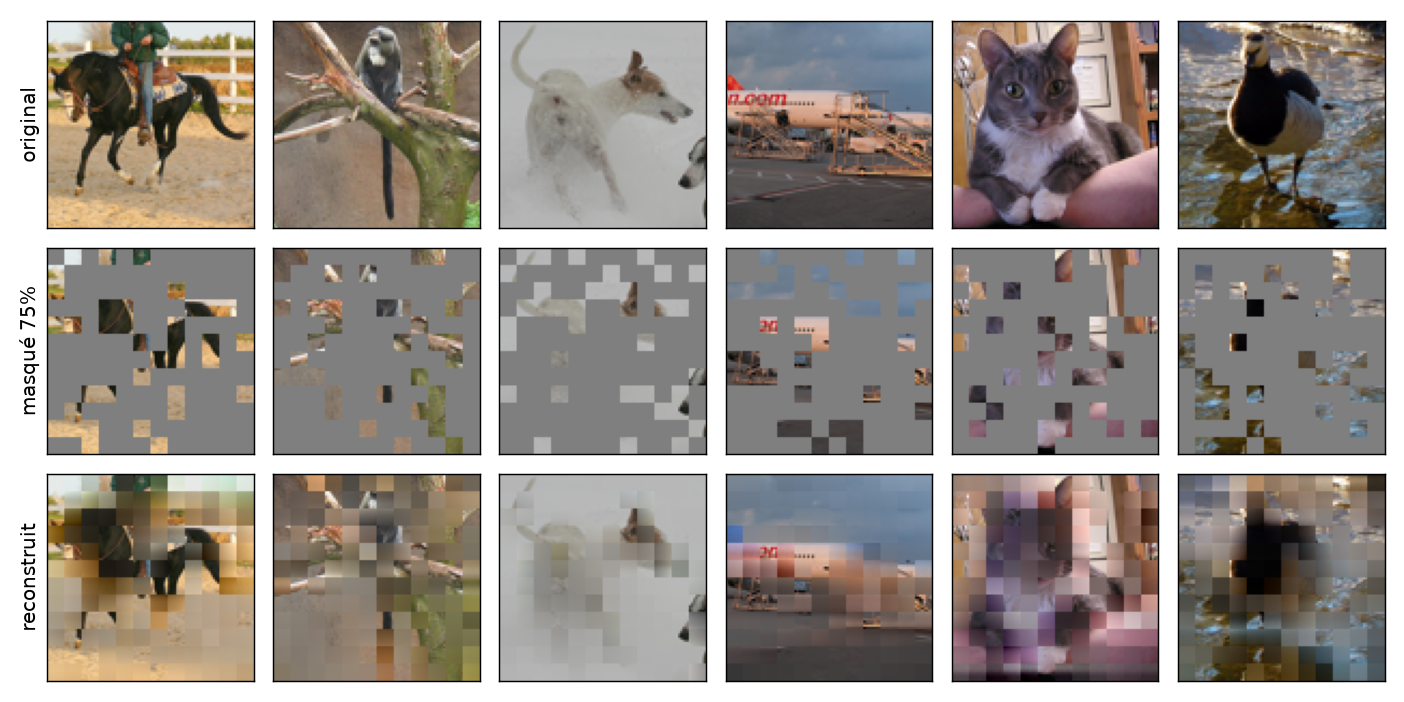
\includegraphics[width=0.86\textwidth]{figures/reconstruction.png}
\caption{STL-10. Original, image masquée (75\,\%) et reconstruction par le MAE.}
\label{fig:stlrecon}
\end{figure*}

\begin{figure}[tbp]
\centering
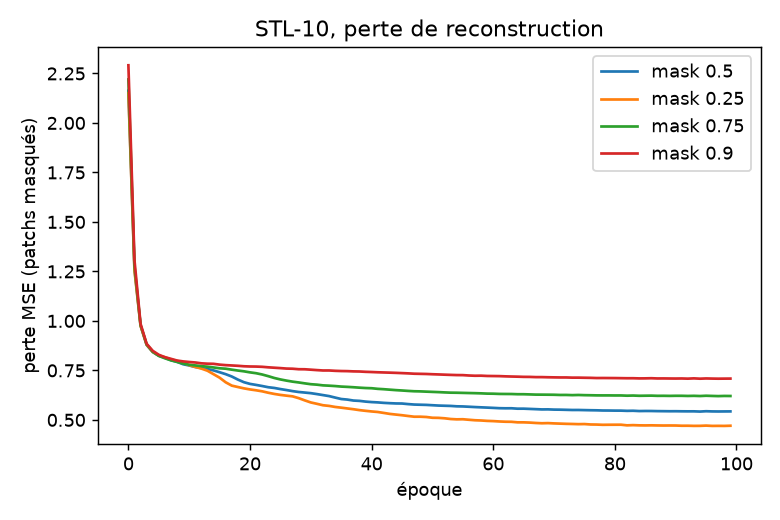
\includegraphics[width=\linewidth]{figures/loss_curves.png}
\caption{STL-10 : perte de reconstruction par taux de masquage. Un taux plus faible donne une tâche
plus facile ; les pertes ne sont pas comparables entre taux, seule la sonde mesure la qualité.}
\label{fig:loss}
\end{figure}

\begin{figure}[tbp]
\centering
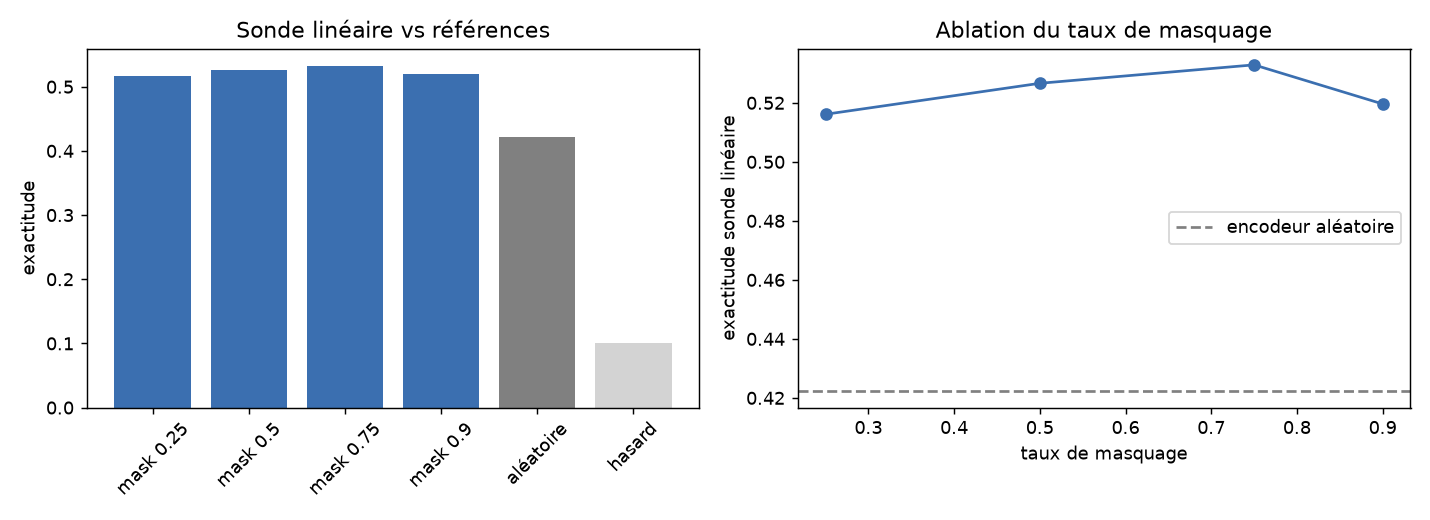
\includegraphics[width=\linewidth]{figures/probe_ablation.png}
\caption{STL-10. Exactitude de la sonde par taux de masquage, contre l'encodeur aléatoire et le
hasard.}
\label{fig:probe}
\end{figure}

\section{Discussion}

\paragraph{Choix de conception.}
Le schéma retenu est le pré-norm, $x \leftarrow x + \mathrm{MHA}(\mathrm{LN}(x))$ puis
$x \leftarrow x + \mathrm{MLP}(\mathrm{LN}(x))$, plutôt que le post-norm présenté en cours : il
conserve un chemin résiduel direct et stabilise l'entraînement en profondeur. L'encodeur n'intègre
pas les tokens masqués : il ne traite qu'un quart des tokens, ce qui réduit le calcul, et ne voit
que de vrais patchs, ce qui évite un écart entre pré-entraînement et déploiement \cite{he2022mae}.
La cible est normalisée par patch, ce qui améliore la qualité des représentations d'après
\cite{he2022mae} (effet non ré-ablaté ici) et impose de dénormaliser les prédictions pour afficher
les reconstructions. Enfin, écrire la rétropropagation à la main sur un simple backend de tableaux
oblige à comprendre chaque gradient, tout en gardant l'accélération GPU.

\paragraph{Limites.}
Le régime est très éloigné de celui de l'article d'origine : un encodeur d'un million de paramètres
contre des centaines de millions, des milliers d'images contre plus d'un million, et un entraînement
court. Les reconstructions, plus fines qu'avec des patchs $16\times 16$, restent floues là où la
perte quadratique pénalise peu les hautes fréquences. Les chiffres proviennent d'une seule graine.
Sur NEU, les textures de défauts sont déjà assez séparables, si bien qu'un encodeur aléatoire obtient
une exactitude élevée et que l'apport du pré-entraînement se lit surtout à faible nombre
d'étiquettes. La rétropropagation manuelle n'est pas en cause : elle est validée par différences
finies.

\section{Conclusion}

Un MAE a été réimplémenté de bout en bout, avec une rétropropagation entièrement manuelle et
vérifiée, torch ne servant que de bibliothèque de tableaux sur GPU. Sur STL-10, le pré-entraînement
dépasse un encodeur aléatoire et l'ablation du taux de masquage illustre, à petite échelle, l'étude
de l'article. Sur un jeu de données industriel de défauts d'acier, le même modèle classe six types
de défauts et montre l'intérêt du pré-entraînement auto-supervisé quand les étiquettes sont rares.

\small
\begin{thebibliography}{99}
\bibitem{he2022mae} K. He et al. \emph{Masked Autoencoders Are Scalable Vision Learners}. CVPR, 2022.
\bibitem{dosovitskiy2021vit} A. Dosovitskiy et al. \emph{An Image is Worth 16x16 Words}. ICLR, 2021.
\bibitem{vaswani2017attention} A. Vaswani et al. \emph{Attention Is All You Need}. NeurIPS, 2017.
\bibitem{devlin2019bert} J. Devlin et al. \emph{BERT}. NAACL, 2019.
\bibitem{bao2021beit} H. Bao, L. Dong, F. Wei. \emph{BEiT}. arXiv:2106.08254, 2021.
\bibitem{vincent2010dae} P. Vincent et al. \emph{Stacked Denoising Autoencoders}. JMLR, 2010.
\bibitem{kingma2015adam} D. Kingma, J. Ba. \emph{Adam}. ICLR, 2015.
\bibitem{loshchilov2019adamw} I. Loshchilov, F. Hutter. \emph{Decoupled Weight Decay Regularization}.
ICLR, 2019.
\bibitem{song2013} K. Song, Y. Yan. \emph{A noise robust method based on completed local binary
patterns for hot-rolled steel strip surface defects}. Applied Surface Science, 2013.
\bibitem{he2020} Y. He et al. \emph{An end-to-end steel surface defect detection approach}. IEEE TIM,
2020.
\bibitem{bhatt2021} P. M. Bhatt et al. \emph{Image-Based Surface Defect Detection Using Deep
Learning: A Review}. ASME JCISE, 2021.
\bibitem{tang2023} B. Tang et al. \emph{Review of surface defect detection of steel products}. IET
Image Processing, 2023.
\end{thebibliography}

\end{document}
